\documentclass[tikz,border=3pt]{standalone}
\usepackage{pgfplots}
\pgfplotsset{compat=1.18}

\begin{document}
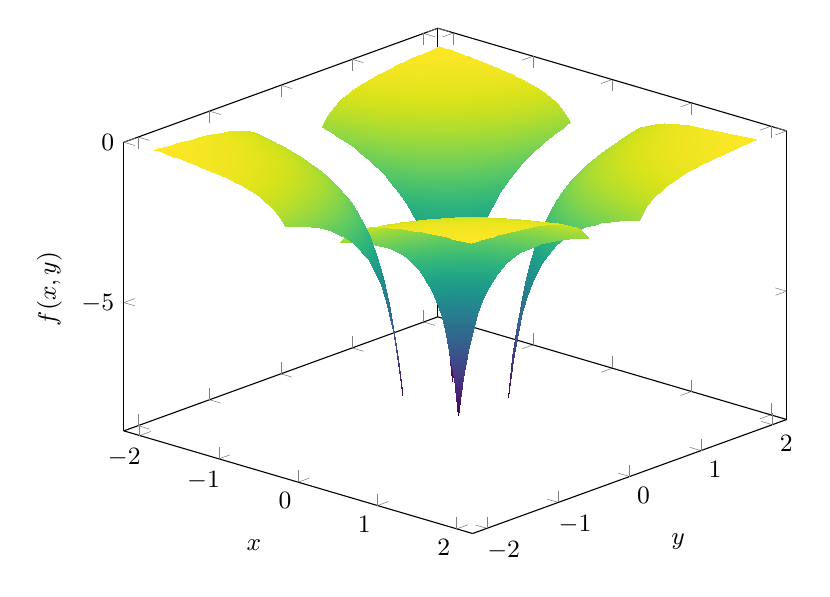
\begin{tikzpicture}
\begin{axis}[
  width=10cm, height=8cm,
  view={42}{28},
  xlabel={$x$}, ylabel={$y$}, zlabel={$f(x,y)$},
  xmin=-2.2, xmax=2.2, ymin=-2.2, ymax=2.2,
  zmin=-9, zmax=0,
  domain=0.35:2, y domain=0.35:2,
  samples=28, samples y=28,
  colormap/viridis,
  tick label style={font=\small},
  label style={font=\small},
  zlabel style={font=\small},
]
  % Excluding |x|<0.35 and |y|<0.35 keeps every sampled point finite.
  % The four patches show the symmetry across the singular axes.
  \addplot3[surf, shader=interp] {-1/(x*y)};
  \addplot3[surf, shader=interp, domain=-2:-0.35] {-1/(abs(x)*y)};
  \addplot3[surf, shader=interp, y domain=-2:-0.35] {-1/(x*abs(y))};
  \addplot3[surf, shader=interp, domain=-2:-0.35, y domain=-2:-0.35]
    {-1/(abs(x)*abs(y))};
\end{axis}
\end{tikzpicture}
\end{document}
